
	\begin{minipage}{12cm}
		\emph{Dans cet exercice, aucune justification n'est demandée.}
		
		On dispose d’un tableau carré ci-contre partagé en neuf cases blanches de mêmes dimensions qui constituent un motif.
	\end{minipage}
	\hfill
	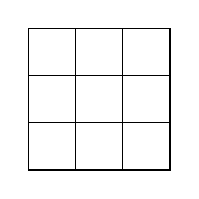
\begin{tikzpicture}[x=6mm,y=6mm, baseline={(current bounding box.center)}]
		\foreach \xy/\c in {(0,0)/white,(1,0)/white,(2,0)/white,
							(0,1)/white,(1,1)/white,(2,1)/white,
							(0,2)/white,(1,2)/white,(2,2)/white}
			\draw[fill=\c, shift={\xy}] (0,0) rectangle (1,1);
	\end{tikzpicture}
		
	\medskip
	
	Quatre instructions A, B, C et E permettent de changer l'aspect de certaines cases, lorsqu'on applique ces instructions. Ainsi:
	
	\begin{tabularx}{\linewidth}{| >{\centering \arraybackslash}m{2cm} | m{8cm} | >{\centering \arraybackslash}X |} \hline
		Instruction & Descriptif & Effet de l'instruction   \\ \hline
		A &   La case centrale du motif est noircie.  & 
		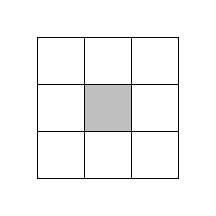
\begin{tikzpicture}[x=6mm,y=6mm, baseline={(current bounding box.center)}]
			\clip (-0.2,-0.2) rectangle (3.2,3.2);
			\foreach \xy/\c in {(0,0)/white,(1,0)/white,(2,0)/white,
				(0,1)/white,(1,1)/gray!50,(2,1)/white,
				(0,2)/white,(1,2)/white,(2,2)/white}
			\draw[fill=\c, shift={\xy}] (0,0) rectangle (1,1);
		\end{tikzpicture}  \\ \hline
		B &   Dans le motif, la case en bas à gauche et la case en haut à droite sont noircies. & 
				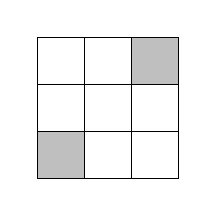
\begin{tikzpicture}[x=6mm,y=6mm, baseline={(current bounding box.center)}]
			\clip (-0.2,-0.2) rectangle (3.2,3.2);
			\foreach \xy/\c in {(0,0)/gray!50,(1,0)/white,(2,0)/white,
				(0,1)/white,(1,1)/white,(2,1)/white,
				(0,2)/white,(1,2)/white,(2,2)/gray!50}
			\draw[fill=\c, shift={\xy}] (0,0) rectangle (1,1);
		\end{tikzpicture}  \\ \hline
		
		C &   Dans le motif, la case médiane à gauche et la case médiane à droite sont noircies. & 
				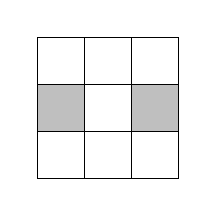
\begin{tikzpicture}[x=6mm,y=6mm, baseline={(current bounding box.center)}]
			\clip (-0.2,-0.2) rectangle (3.2,3.2);
			\foreach \xy/\c in {(0,0)/white,(1,0)/white,(2,0)/white,
				(0,1)/gray!50,(1,1)/white,(2,1)/gray!50,
				(0,2)/white,(1,2)/white,(2,2)/white}
			\draw[fill=\c, shift={\xy}] (0,0) rectangle (1,1);
		\end{tikzpicture}  \\ \hline
		
		
		E &  Les couleurs du motif sont inversées: les cases blanches deviennent noires et les les cases noires deviennent blanches.&
				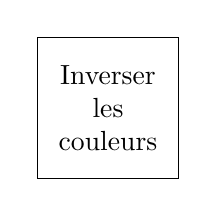
\begin{tikzpicture}[x=6mm,y=6mm, baseline={(current bounding box.center)}]
			\clip (-0.2,-0.2) rectangle (3.2,3.2);
			\draw[] (0,0) rectangle (3,3) ;
			\node (t) at (1.5,1.5) [text width=1.5cm, align=center] {Inverser\\ les\\ couleurs};
		\end{tikzpicture}  \\ \hline

	\end{tabularx}

\smallskip

\emph{Remarque} : si une case du motif est déjà noire et une instruction demande de la noircir, alors cette case ne change pas de couleur et reste noire à la suite de cette instruction.
	
\smallskip
	
\emph{Exemples} : à partir d’un motif dont toutes les cases sont blanches:
	
		\begin{tabularx}{\linewidth}{X c @{\hspace{5mm}}|@{\hspace{5mm}} X c} 
		la suite d'instructions A C permet d'obtenir ce motif &
		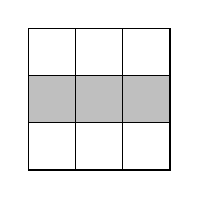
\begin{tikzpicture}[x=6mm,y=6mm, baseline={(current bounding box.center)}]
			\foreach \xy/\c in {(0,0)/white,(1,0)/white,(2,0)/white,
								(0,1)/gray!50,(1,1)/gray!50,(2,1)/gray!50,
								(0,2)/white,(1,2)/white,(2,2)/white}
				\draw[fill=\c, shift={\xy}] (0,0) rectangle (1,1);

		\end{tikzpicture}&
		la suite d'instructions A C E permet d'obtenir ce motif &
		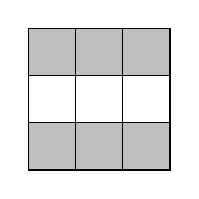
\begin{tikzpicture}[x=6mm,y=6mm, baseline={(current bounding box.center)}]
			\foreach \xy/\c in {(0,0)/gray!50,(1,0)/gray!50,(2,0)/gray!50,
								(0,1)/white,(1,1)/white,(2,1)/white,
								(0,2)/gray!50,(1,2)/gray!50,(2,2)/gray!50}
					\draw[fill=\c, shift={\xy}] (0,0) rectangle (1,1);
		\end{tikzpicture}\\		
	\end{tabularx}

\medskip

Pour chacune des questions suivantes, on dispose au départ d’un motif dont toutes les cases sont blanches.
	
	\begin{enumerate}
		\item Représenter le motif obtenu avec la suite d'instructions A B.
		
		\item \begin{minipage}[t]{11 cm}
Parmi les quatre propositions suivantes, deux propositions permettent d'obtenir le motif ci-contre. Lesquelles ?
			
			\smallskip 
			
\begin{tabularx}{\linewidth}{*{2}{>{\bfseries Proposition \no }l <{ :} @{~} X}}
1 & A B C   & 3 & B C E C\\ [6pt]
2 & C E     & 4 & C A E A\\
\end{tabularx}
		\end{minipage}
		\hfill
		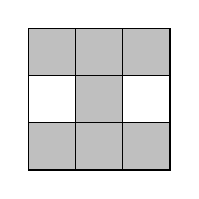
\begin{tikzpicture}[x=6mm,y=6mm, baseline={(0,1.6)}]
			\foreach \xy/\c in {(0,0)/gray!50,(1,0)/gray!50,(2,0)/gray!50,
								(0,1)/white,(1,1)/gray!50,(2,1)/white,
								(0,2)/gray!50,(1,2)/gray!50,(2,2)/gray!50}
				\draw[fill=\c, shift={\xy}] (0,0) rectangle (1,1);
		\end{tikzpicture}
		
		\item \begin{minipage}[t]{11 cm}
Donner une suite d'instructions qui permet d'obtenir le motif ci-contre.	
		\end{minipage}
		\hfill
%		\begin{tikzpicture}[x=6mm,y=6mm, baseline={(0,0.8)}]
%			\foreach \xy/\c in {(0,0)/gray!50,(1,0)/gray!50,(2,0)/white,
%								(0,1)/gray!50,(1,1)/white,(2,1)/gray!50,
%								(0,2)/white,(1,2)/gray!50,(2,2)/gray!50}
%			\draw[fill=\c, shift={\xy}] (0,0) rectangle (1,1);
%		\end{tikzpicture}
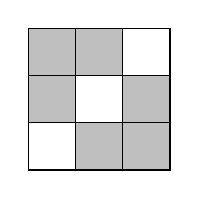
\begin{tikzpicture}[x=6mm,y=6mm, baseline={(0,0.8)}]
			\foreach \xy/\c in {(0,0)/white,(1,0)/gray!50,(2,0)/gray!50,
								(0,1)/gray!50,(1,1)/white,(2,1)/gray!50,
								(0,2)/gray!50,(1,2)/gray!50,(2,2)/white}
			\draw[fill=\c, shift={\xy}] (0,0) rectangle (1,1);
		\end{tikzpicture}
	\end{enumerate}

\bigskip

